\chapter{Extension of cgNA$+$ parameter sets for epigenetically modified DNA} \label{c6}

%~\cite{peters2010dna,peters2014mechanical} -- review on DNA mechnics modified and unmodif --
% -- {DNA} methylation landscapes: provocative insights from epigenomics ~\cite{suzuki2008dna} \\
% -- ~\cite{miranda2007dna} --  title={{DNA} methylation: the nuts and bolts of repression},\\
% -- ~\cite{chandler1988hypomethylation}, Hypomethylation of {DNA} in the regulation of gene expression \\
% -- ~\cite{cedar2009linking} Linking {DNA} methylation and histone modification: patterns and paradigms \\
% -- ~\cite{perez2012impact} : demonstrated that \cpg steps display unique physical property, specially in the cintext of /cpg islands that severely changes  on methylation -- check out this work ...in notability \\
% -- ~\cite{dantas2015evolving},Evolving insights on how cytosine methylation affects protein--{DNA} binding \\

%\rs{need to discuss MBD, CpG islands at some point, disubs or hemi ..which are popolar} \\
%\rs{mention somehwrere that modified DNA means bla bla} \\

% ~\cite{teng2018effect} -- effect of methylation on DNA mechanics
% ~\cite{hognon2019cooperative} --- methylated is in major groove -- thus modifying groove accessibility 
% Lazarovici et al.~\cite{lazarovici2013probing} found that the DNase-\rom{1} cleavage rate is correlated with the minor groove width. Furthermore, for the same kind of genome, cleavage activity adjacent to \cpg steps increases approximately eight times on cytosine methylation due to minor groove narrowing.
%~\cite{battistini2021impact,carvalho2014understanding}
%~\cite{severin2013effects} -- could regulate gene expression through altering mechanical properties of DNA, single-molecule force microscopy experiments with steered MD simulations and showed that cytosine methylation and hydroxymethylation alter the mechanical properties of DNA, thus facilitating strand separation involvement in gene regulation.
%~\cite{munzel2010quantification}
%~\cite{guibert2013functions}
%~\cite{carvalho2014understanding} -- both extent and position of modification have significant effects on structural variations, change in Twist, Tilt and Roll is observed. 

% The term \say{epigenetics} coined by C. H. Waddington in 1942 literally means \say{in addition to} genetics and 
% is formally defined~\cite{berger2009operational} as \say{An epigenetic trait is a stably heritable phenotype resulting from changes in a chromosome without alterations in the DNA sequence}.
% The most studied epigenetic modifications include DNA methylation, non-coding RNAs, and histone modification that can change the gene expression without changing its DNA sequence.
% Epigenetics has implications in gene silencing~\cite{kass1997does,cedar2009linking,pennings2005dna}, X-chromosome inactivation~\cite{goto1998regulation}, and in humans, epigenetic aberrations are associated with diseases such as cancer, autoimmune disease, and neurodevelopmental disorders~\cite{portela2010epigenetic,kulis2010dna} and, therefore, is a great interest for research.
% Moreover, some of these aberrations are reversible and targeted in therapeutic approaches ~\cite{kelly2010epigenetic}.

The primary focus of this chapter is DNA base modifications, in particular, methylation or hydroxymethylation at the $5$-position of cytosine in \cpg steps.
DNA methylation, regulated by the DNA methyltransferase enzyme, plays a pivotal role in several biological processes, such as X-chromosome inactivation and genomic imprinting, while aberrations in methylation patterns are often associated with diseases such as cancer~\cite{portela2010epigenetic,kulis2010dna}.
Around 70-80\% of the \cpg steps are methylated in mammalian cells~\cite{jabbari2004cytosine} except for the \cpg islands (dominantly present in the gene promoter regions).
In general, methylation of \cpg steps in promoter regions is anti-correlated with gene expression~\cite{cedar2009linking,pennings2005dna}. 
It is believed that \cpg methylation reduces the flexibility of DNA~\cite{cortini2016physics,perez2012impact,portella2013understanding} and thus, reduces the ability of DNA to interact with transcription factors, modulates DNA accessibility, and makes them less prone to wrap around nucleosomes.
However, recent works have shown contrasting findings with hypermethylation related to increased DNA flexibility~\cite{pongor2017optical,shon2019submicrometer,marin2019dna,liebl2019methyl}.
It highlights that the influence of base modifications on DNA mechanics is complex and depends on the extent and position of base modifications.
Moreover, Rausch et al.~\cite{rausch2021cytosine} showed \textit{in vivo} and \textit{in vitro} experiments that cytosine methylation stabilizes double-stranded DNA (dsDNA) helix by increasing its melting temperature and resisting enzymatic activities toward dsDNA, therefore, suggesting its crucial role in regulating dsDNA access and genomic processes.

In comparison to DNA methylation, DNA hydroxymethylation has received much less attention because of its relatively low abundance in genomes and the lack of experimental techniques to resolve hydroxymethylated C from methylated C.
Hydroxymethylated C is the result of oxidation of methylated cytosine in \cpg steps catalyzed by ten-eleven translocation proteins~\cite{tahiliani2009conversion}. 
DNA hydroxymethylation has been observed in the genomic regions of many organisms, in particular, prevalent in mammalian brain cells~\cite{munzel2010quantification} and embryonic stem cells.
The disturbed hydroxymethylation pattern of DNA cytosine may result in disordered cell function and, thus, in different types of cancers, e.g., myeloid cancers~\cite{ko2010impaired}.

There are both experimental and theoretical evidence that these modifications bring about changes at the structural
level~\cite{b1favour,battistini2021impact,lefebvre1996solution,rao2018systematic,carvalho2014understanding} as well as modulate overall mechanics~\cite{severin2011cytosine,ngo2016effects,geahigan2000dynamic,jimenez2014unmethylated,carvalho2014understanding,severin2013effects}.
However, these studies lack consensus on their findings. 
It is probably because alterations in dsDNA properties on base modifications are highly dependent on the modification level and the flanking sequence.
Thus, a systematic investigation of how epigenetic base modifications influence dsDNA mechanics is required. 
A coarse-grained model such as cgNA$+$, which has been demonstrated to be indistinguishably accurate in predicting the mechanics (equilibrium shape and stiffness) of dsDNA, dsRNA, and DRH, will be highly beneficial to obtain insights into the role of epigenetic base modifications in dsDNA mechanics and, thus, better understand its function in biology.
This chapter discusses the extension of the cgNA$+$ model for epigenetically modified dsDNA, in particular, for sequences containing methylated and hydroxymethylated \cpg \ steps.

Details of all the codes and data used in this chapter are provided \cref{app6}. 

\section{cgNA$+$ for epigenetically modified dsDNA}
This section describes the extension of cgNA$+$ to predict the Gaussian pdfs for sequences containing methylated and hydroxymethylated \cpg steps.
First, we describe the epigenetic base modifications in dsDNA and introduce a notation for modified cytosine. 
We then describe the training sequences used to train the cgNA$+$ parameters for modified base-pair steps. Lastly, we discuss the training of the cgNA$+$ parameter set $\mathcal{P}_{\text{Met/Hmet}}$ which in combination with existing $\mathcal{P}_{\text{DNA}}$ will allow predicting groundstate and stiffness matrix for any sequence containing methylated/hydroxymethylated \cpg steps. 

\subsection{Epigenetic modifications in DNA bases}
The most common epigenetic modifications in DNA bases are methylation and hydroxymethylation of cytosine at the 5--position. 
The chemical structures of these modified cytosines are shown in \cref{c1:fig1}.
Other base modifications, such as 5-formyl-C, 5-carboxyl-C, and N6-methyl-A, are comparatively rare in biology.
Furthermore, most often, cytosine methylation or hydroxymethylation occurs at \cpg dinucleotide steps, which can be di-substituted if both strands are symmetrically modified or hemi-substituted if only one of the strands is asymmetrically modified.
This work focuses only on cytosine modification in \cpg steps.

\subsection{Alphabets for epigenetically modified cytosine}
In this work, to describe the DNA sequence, we have used the standard alphabets A, T, C, and G for bases. 
However, the notation for hydroxymethylated or methylated cytosines is not standardized.
This thesis uses the letter M for 5-methylated-cytosine, and N for Guanine when complementary cytosine is methylated.
Similarly, letters H and K are used for 5-hydroxymethylated-cytosine and Guanine complementary to 5-hydroxymethylated-cytosine, respectively.
For example, MN represents symmetrically methylated cytosine on both strands, CN denotes asymmetrically methylated cytosine on the Crick (complementary) strand, and MG denotes asymmetrically methylated cytosine on the Watson (reading) strand.
Following this notation, M and H are complementary bases to N and K, respectively, and dimer steps such as MN, NM, HK, and KH are palindromes.
Thus, for modified DNA, any sequence can be described using alphabets $X_i \in$ \{A, T, C, G, M, N, H, K\}.
%Note that this thesis focuses on double-stranded nucleic acids (dsNAs) and all the following discussion on epigenetically modified DNA is pertinent to dsDNA. 

\subsection{Training library}
As discussed in \cref{c2}, cgNA$+$ is a coarse-grained model trained on MD simulations for a set of sequences called the training library.
To train the cgNA$+$ parameter set that allows cytosine base modifications in \cpg steps, we have used an extensive library of 12 sequences provided in \cref{epilib}.
The libraries are denoted as \Lbm \ and \Lbh \ containing sequences with methylated and hydroxymethylated \cpg steps.
The key features of these libraries include: (a) all the training sequences are palindromes, which allows quantifying the convergence of the MD simulations (refer to \cref{c3} for details), (b) contains both di-substituted and hemi-substituted \cpg steps in diverse sequence contexts, and (c) contains various combinations on modified \cpg steps (for instance, MNMN or MGCN or CNMG in \Lbm).
Thus, training sequences are designed optimally to have minimal sequences in the library with various combinations of modified base-pair steps in diverse sequence contexts.
It should be noted that library design is a crucial step in the cgNA$+$ model.
The training data must have sufficient diversity for any data-driven model to ensure accurate/reasonable predictions for unseen samples.
In the case of the cgNA$+$ model, as discussed in \cref{c4:s1}, lack of diversity in the training sequence may lead to a non-positive reconstruction of the stiffness matrix as observed in some dsDNA sequences with non-GC ends~\cite{patelithesis}. 
This problem was solved using a comprehensive library with diverse contexts for non-GC ends (refer \cref{c4:s1,endlib}).
A similar problem was also encountered during experimentation of modified parameter set; in particular, a parameter set trained on sequences without various combinations of modified \cpg steps (i.e., without using sequence indices 9 to 12) predicts a non-positive definite stiffness matrix for sequences with adjacent repeats of modified \cpg steps (for instance, GC$\cdots$ATMNCNMG$\cdots$GC).
It again highlights how crucial library design is for the cgNA$+$ model.

Lastly, MD simulations for all sequences in \Lbm \ and \Lbh \ are performed using the same MD protocol used for dsDNA with additional force-field parameters for modified cytosine. 
Details of MD protocol and post-processing are provided in \cref{c3:s2,c3:s4}, respectively.

\subsection{Training of cgNA$+$ parameter set to allow epigenetically modified cytosine}\label{c6:epi_param}
The cgNA$+$ model requires a parameter set containing dimer-dependent blocks for stiffness matrix and stress vector to predict a Gaussian pdf for a given sequence.
In this work, the aim is to extend $\mathcal{P}_{\text{DNA}}$ (defined in \cref{c4:eq2_DNA}) that allows prediction of Gaussian pdf for any sequence containing methylated or hydroxymethylated \cpg steps.
We started with the approximation that the parameter blocks for the unmodified base-pair steps remain the same.% for a sequence containing modified \cpg steps.
It implies that we need to estimate parameters only for \{MN, NM, MG, CN, AM, TM, CM, GM, NA, NG, NT, NC\} dimer steps out of which \{MN, NM, MG, AM, TM, CM, GM\} dimer steps are independent.
Similarly, to allow hydroxymethylated \cpg steps, parameters for \{HK, KH, HG, AH, TH, CH, GH\} dimer steps are required, while for the dependent dimers, the parameters can be obtained using the CW symmetry relation defined in \cref{c2:eq_CW_in_Prm}.
Thus, for any sequence containing modified \cpg steps, the groundstate and stiffness matrix can be predicted using cgNA$+$ model with a combination of $\mathcal{P}_{\text{DNA}}$ and $\mathcal{P}_{\text{Met/Hmet}}$ given as
\begin{equation}
\mathcal{P}_{\text{Met/Hmet}} = \{ \sigma^{\XY}, \K^{\XY} \} \in   [\R^{42}]^{7} \times [\R^{42 \times 42}]^{7},
\label{c6:eq1_prm_met}
\end{equation}
where $\XY \in$ \{MN, NM, MG, AM, TM, CM, GM\} for $\mathcal{P}_{\text{Met}}$ and $\XY \in$ \{HK, KH, HG, AH, TH, CH, GH\} for $\mathcal{P}_{\text{Hmet}}$. \vfill \clearpage

Once again, it must be noted that $\mathcal{P}_{\text{Met/Hmet}}$ only allows modified \cpg steps, not modified \gpc steps. 
Taking the example of dsDNA methylation, NM and GM (or NC) steps are not allowed.
It is contradictory and confusing, as $\mathcal{P}_{\text{Met}}$ already contains parameters for these dimer steps.
This is because NM and GM (or NC) steps naturally arise in various combinations of methylated \cpg steps which are allowed.
For example, NM and GM steps are present in repeated combinations of methylated \cpg steps such as MNMN/CNMN/CNMG and MGMN/MGMG, respectively.
Therefore, to write precisely, XNMZ and XGMZ (or XNCZ) steps are not allowed where X $\in$ \{A, T, G\} and Z $\in$ \{A, T, C\} as these steps represent methylated \gpc step.
Moreover, in the current version of cgNA$+$, a sequence containing both hydroxymethylated and methylated \cpg steps is only allowed as input when they are not present adjacent to each other.
%Also, $\mathcal{P}_{\text{Met/Hmet}}$ do not contain parameters for modified \cpg steps at the end of sequences.

Lastly, since we already have parameters for NM and GM, one can contemplate using these parameters to predict Gaussian pdf for a sequence containing methylated \gpc steps. 
Such an exercise might lead to a non-positive definite stiffness matrix for that sequence.
The only explanation justifying the non-positive definite reconstruction of such sequences is that the training library does not contain any such example cases.
It again highlights the importance of training library design.
However, it leads to a technical issue in $\mathcal{P}_{\text{Met/Hmet}}$ parameter sets. As once the cgNA$+$ parameter set is computed, the next step is to search the block elements in the null space to check whether dimer stiffness blocks in the parameter set are positive-definite (refer to \cref{c2:sec4,c2:s4:sb6}) which ensure a positive-definite stiffness matrix for any given sequence.
However, in the case of $\mathcal{P}_{\text{Met/Hmet}}$, we already know that it is not possible to find such block elements as sequences containing XNMZ and XGMZ (or XNCZ) steps where X $\in$ \{A, T, G\} and Z $\in$ \{A, T, C\} give non-positive definite stiffness matrix.
The next best check to confirm positive-definite reconstruction for any sequence is to examine the reconstructed stiffness matrix for a large ensemble of sequences and hope that for any other sequences, not in this ensemble; the cgNA$+$ model will predict positive-definite Gaussian pdf.
We checked the definiteness of the predicted stiffness matrix for (a) all 16mers in GC ends and (b) $10^8$ random sequences of length varying from 16 to 300 bps containing at least one modified \cpg steps. 
This test was performed individually for both $\mathcal{P}_{\text{Met/Hmet}}$, and positive-definite stiffness matrices were obtained for all sequences. 
Note that for dsDNA/dsRNA/DRH, before searching for block elements in null-space, we reconstruct all sequences of length 4-10 and check the definiteness of the stiffness matrix. 
In all the cases (RNA/DNA/DRH), even if stiffness matrices for all hexamers for a given parameter set are positive definite, we were always able to find positive-definite dimer stiffness parameter blocks.
It further establishes trust in $\mathcal{P}_{\text{Met/Hmet}}$ that for any given sequence containing modified \cpg steps, cgNA$+$ reconstruction will be positive-definite, however, it can not be guaranteed as in the case of $\mathcal{P}_{\text{DNA/RNA/DRH}}$. 


%%%%%%%%%%%%%%%%%%%%%%%%%%%%%%%%%%%%%%%%%%%%%%%%%%%%
%%%%%%%%%%%%%%%  NEXT SECTION  %%%%%%%%%%%%%%%%%%%%%
%%%%%%%%%%%%%%%%%%%%%%%%%%%%%%%%%%%%%%%%%%%%%%%%%%%%

\section{cgNA$+$ reconstructions and associated modeling errors}\label{c6:s2}
This section is similar to the previous discussion in \cref{c4:s3} and investigates the performance of the cgNA$+$ model in predicting groundstate and stiffness for dsDNA sequences with epigenetic base modifications.
In particular, we have tested the cgNA$+$ model on sequences that are not part of the training sequences for $\mathcal{P}_{\text{Met/Hmet}}$. 

\subsection{Test library}
To assess the cgNA$+$ model, we have simulated several test sequences (listed in \cref{epilib}) using the same MD protocol as used for the training sequences.
These test sequences are designed carefully to critically examine various aspects of the cgNA$+$ model's predictive capability. 
For instance, sequence index 18 in \Lbm \ or \Lbh \ is the symmetric modified (methylated or hydroxymethylated) version of sequence index 20 in \Lbdna \ at the interior \cpg step.
This sequence allows to check how well cgNA$+$ captures the change in groundstate of this sequence \say{GCGGATTA\textbf{CG}CAGGC} upon symmetric modification of the \cpg step (highlighted in bold).
Furthermore, sequence index 24 in \Lbdna \ is a typical \cpg island, and to check the effect of \cpg methylation/hydroxymethylation, we have simulated sequence indices 19 to 21 (in \Lbh \ or \Lbm) which are differently modified variants of the same \cpg islands.

\subsection{Reconstruction error in cgNA$+$ model}\label{c6:res_error_sec}
In this subsection, first, we have plotted the groundstate for a few selected sequences along with the observed MD estimates to visualize the model accuracy and highlighted that the cgNA$+$ model captures non-local changes (i.e., the change in groundstate is propagated to the neighboring base-pair steps) in groundstate due to base modifications in the sequence (notably base modification can be considered as a smaller change than point mutation).
In \cref{c6:figure1}(a), we have compared the groundstate of unmethylated and methylated versions of \say{GCGGATTA\textbf{CG}CAGGC} (symmetric methylation at the highlighted \cpg step). 
First, note that the change in groundstate due to methylation of one \cpg step is highly non-local. 
Furthermore, it can be observed in the plot that the average shape in MD simulations and groundstate predicted by the cgNA$+$ model are indistinguishable and, thus, the cgNA$+$ model accurately captures non-local changes in groundstate on methylation of \cpg steps. 
This is further quantified as the reconstruction error in terms of the Mahalanobis distance and is equal to $\approx 0.0027$ \AA$^2$ or (rad/5)$^2$ for test sequences (refer \cref{c6:tab2_errors}(a)).
An analogous plot for hydroxymethylation of the highlighted \cpg step in \say{GCGGATTA\textbf{CG}CAGGC} is provided in \cref{c6:figure1}(b), and similar conclusions can be drawn about the accuracy of the model and the impact of \cpg hydroxymethylation on groundstate.

\begin{figure}
  \begin{subfigure}{15cm}
    \centering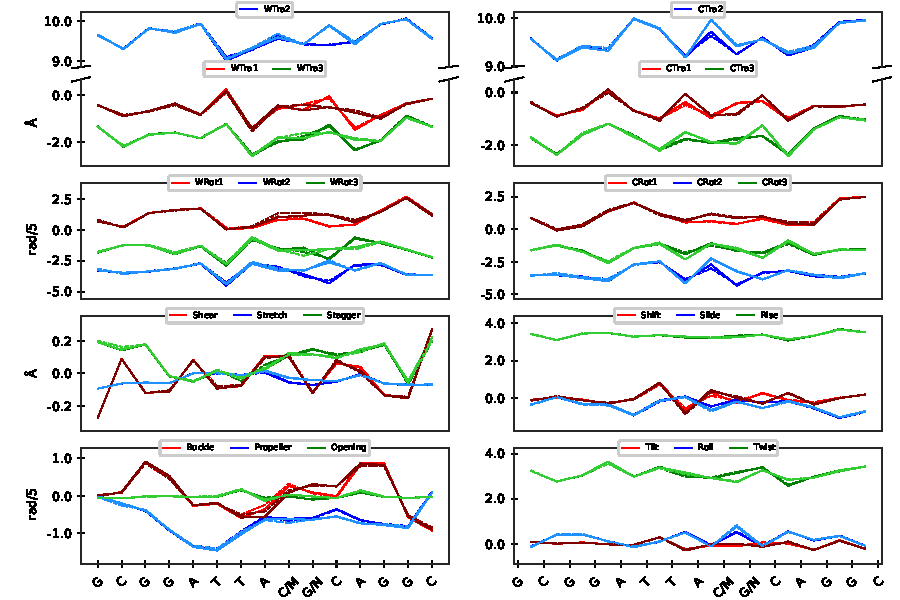
\includegraphics[width=15cm]{images/compare_seq_MDNA_DNA_18.pdf}
    \caption{Methylation of \cpg step}
  \end{subfigure}
  \begin{subfigure}{15cm}
    \centering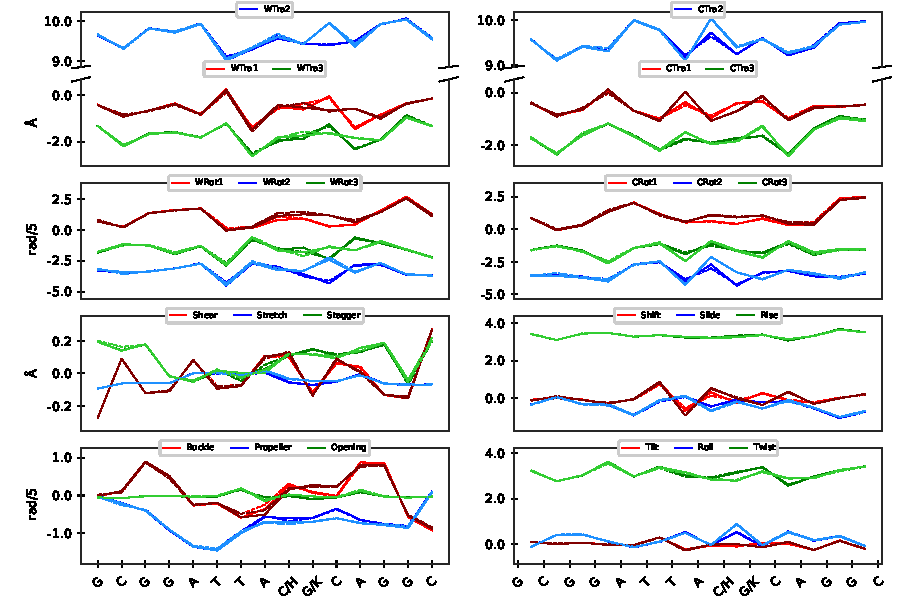
\includegraphics[width=15cm]{images/compare_seq_HDNA_DNA_18.pdf}
    \centering\caption{Hydroxymethylation of \cpg step}
  \end{subfigure}
\centering\caption{Groundstate coordinates (elements of $w$) for (a) sequence index 20  in \Lbdna \ (red, blue, and green as shown in legend) and 18 in \Lbm \ (in dark red, dark blue, dark green) and (b) sequence index 20 in \Lbdna \ (red, blue, and green as shown in legend) and 18 in \Lbh \ (in dark red, dark blue, dark green). The figure highlights the cgNA$+$ model accuracy in predicting the non-local change in groundstate due to (a) methylation and (b) hydroxymethylation of \cpg step. MD estimates are in solid lines while dashed lines are cgNA$+$ reconstructions.}
\label{c6:figure1}
\end{figure}

\begin{figure}
  \begin{subfigure}{15cm}
    \centering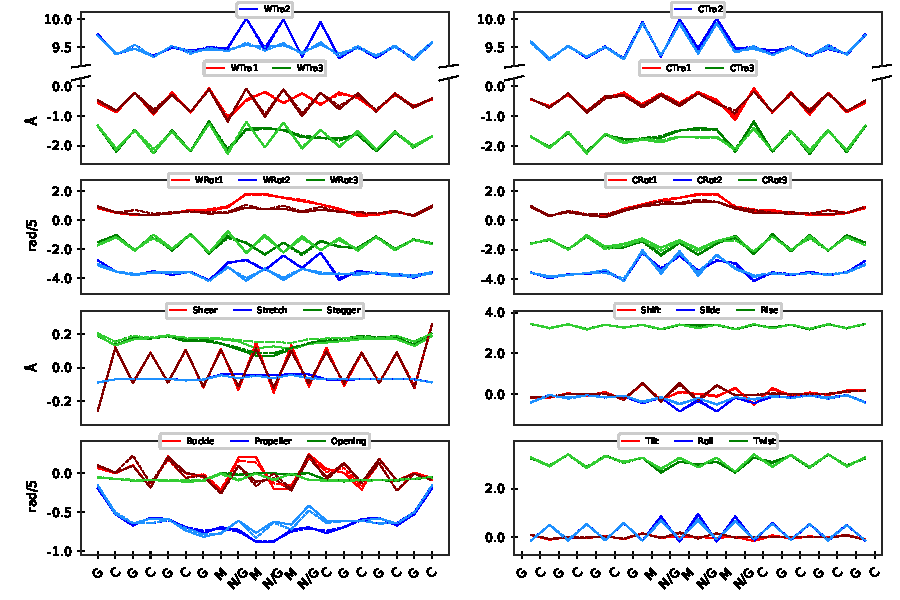
\includegraphics[width=15cm]{images/cpg_islands_2.pdf}
    \centering\caption{Symmetric vs asymmetric methylation of \cpg islands}
  \end{subfigure} 

  \begin{subfigure}{15cm}
    \centering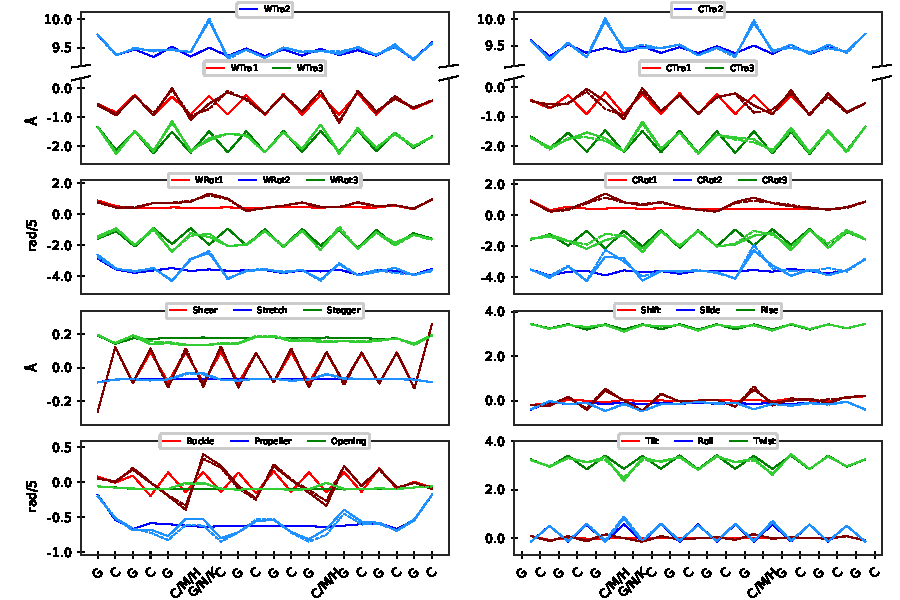
\includegraphics[width=15cm]{images/cpg_islands_1.pdf}
    \centering\caption{Symmetric and asymmetric methylation and hydroxymethylation of \cpg islands}
  \end{subfigure}
\centering\caption{Groundstate coordinates (elements of $w$) for (a) sequence index 19 \ (red, blue, and green as shown in legend) and 20 in \Lbm \ (in dark red, dark blue, dark green) where MD estimates are in solid lines while dashed lines are cgNA$+$ reconstructions, and (b) sequence index 20 in \Lbdna \ (red, blue, and green as shown in legend) and 21 in \Lbm \ (in solid lines) and \Lbh \ (in dashed lines) in dark red, dark blue, dark green. The figure highlights (a)  the cgNA$+$ model accuracy in predicting change in groundstate due to symmetric and asymmetric methylation of \cpg islands and (b) impact of methylation and hydroxymethylation on groundstate of \cpg islands.}
\label{c6:figure2}
\end{figure}
%\rs{It might be better to explain here in more detail which bases are methylated as the axis label is confusing. The accuracy statement can go safely into the main text....} \\
Furthermore, in \cref{c6:figure2}(a), we have compared the groundstate for monomethylated (asymmetric) and dimethylated (symmetric) typical \cpg islands to highlight the difference in groundstate for two differently substituted \cpg steps. 
% and cgNA$+$ model ability to accurately captures these changes.
It can be observed that asymmetric and symmetric methylation of \cpg steps leads to a significantly different groundstate and the model accurately captures those changes.
Similar results were also observed for asymmetric and symmetric hydroxymethylation of \cpg steps in \cpg islands (not shown in the thesis for brevity). 
%\rs{I read this before, but fail to understand why. The explanation is technical.}
Lastly, we would like to emphasize that internal coordinates for \cpg steps are often multi-modal (refer to \cref{c3:fig_distr_2}) and highly sensitive to flanking sequence context.
So, one can expect a larger reconstruction error in the prediction of groundstate for \cpg steps compared to other dimer steps for dsDNA or, in general, for dsRNA (where internal coordinate distributions are close to Gaussian) due to much complicated and larger conformational space.
Therefore, it again highlights how impressive the cgNA$+$ model is in predicting groundstate for such modified sequences containing \cpg steps.

In the second part, we have quantified the total reconstruction error in the cgNA$+$ model for sequences with epigenetic modifications.
The reconstruction error $\er^{\text{res}}$ (refer to \cref{c2:s5sb3}) for the cgNA$+$ model is defined as the deviation of the predicted Gaussian pdf from the corresponding observed Gaussian pdf in MD simulations and is computed in terms of symmetric KL divergence and symmetric Mahalanobis distance. 
Note that $\er_{\text{KL}}^{\text{res}}$ (reconstruction error in terms of KL divergence) describes the total reconstruction error (both in groundstate and stiffness matrix) in the cgNA$+$ model, while the $\er_{\M}^{\text{res}}$ (reconstruction error in terms of Mahalanobis distance) highlights the difference in the predicted groundstate and MD average shape scaled by stiffness.
In \cref{c6:tab2_errors}(a), we have tabulated the reconstruction errors per degree of freedom, dof (which is $24N-18$, i.e., the number of internal coordinates required to describe a given sequence of length $N$ bp) in the training and test sequences for \Lbm \ and \Lbh.
Firstly, the average reconstruction error in the training sequences in \Lbm \ is 0.0023 and 0.0304 in terms of $\er_{\M}^{\text{res}}$ and $\er_{\text{KL}}^{\text{res}}$, respectively, which is roughly one order of magnitude smaller than the corresponding \textit{scale}, 0.0211 and 0.3378, computed as average pair-wise difference of training sequences (see \cref{c2:s5sb4}) and is a quantification of variation over sequence.
It highlights the precision of the cgNA$+$ model in accurately capturing the non-local sequence-dependent mechanics of dsDNA.
Moreover, the analogous reconstruction errors, $\er_{\text{KL}}^{\text{res}}$ and $\er_{\M}^{\text{res}}$ for the test sequences in \Lbm \ are 0.0025 and 0.0311 which are almost equal to the errors in the reconstruction of the training sequences. 
It comments on the generalizability of the cgNA$+$ model. 
Similar observations can be made for training and test sequences in \Lbh. 
It should be noted that the reconstruction errors obtained here are comparable to the corresponding results for \Lbdna \ (in \cref{c4:tab1_errors}). 
However, the \textit{scale} obtained here for \Lbh \ and \Lbm \ is noticeably smaller than \textit{scale} for \Lbdna \ because the training sequences in \Lbh \ or \Lbm \ are similar to each other than in \Lbdna.

This total reconstruction error in the cgNA$+$ model results from several modeling assumptions in our model, as listed in \cref{c2:sec3} and the error associated with each assumption can be quantified as described in \cref{c2:sec5}.
We have discussed the contributions of various modeling assumptions to the reconstruction error in the following subsections.

\subsection{Approximation error in the training data}\label{c6:converge_error_sec}
The first modeling assumption in the cgNA$+$ model is that the MD time series is fully converged.  
The associated convergence error (referred to as palindromic error) is discussed in \cref{c2:s5sb1}, and details of this error quantification are provided in \cref{c3:s5,c3:tab_con_rest}. 
For the training sequences in \Lbh \ and \Lbm, the average palindromic error in terms of KL divergence $\er_{\text{KL, avg}}^{\text{palin}}$ and Mahalanobis distance $\er_{\M, \ \text{avg}}^{\text{palin}}$ are of the order $10^{-4}$ and $10^{-3}$, respectively, which are approximately two orders smaller than the corresponding \textit{scales}. 



Moreover, in \cref{c3:s6}, we have discussed the distribution of internal coordinates in MD time-series and shown that the distributions for inter base-pair step and phosphate coordinates for dsDNA often deviate from Gaussian behavior and depend on the flanking sequence context.
However, for modeling purposes, we have imposed Gaussianity to the underlying distribution for internal coordinates, leading to an inevitable modeling error. 
We have quantified this modeling error by computing the KL divergence between observed pdf and best-fit Gaussian pdf to the observed pdf and found that except for Wtra1 phosphate coordinate, $\er_{\text{KL}}^{\text{Gauss}}$ is less than \textit{scale}. \clearpage

\clearpage
\begin{table}[H]
\begin{subtable}[h]{1.0\textwidth}
\begin{center}
\begin{small}
\begin{tabular}{ c || c c | c c  }
  \multicolumn{3}{c}{\; \; \; \; \; \; \; \; \; \ \Lbm}& \multicolumn{2}{c}{\Lbh} \\
\hline
  \multicolumn{5}{c}{Training sequences} \\
\hline
Index & $\er_{\M}^{\text{res}}$ & $\er_{\text{KL}}^{\text{res}}$ & $\er_{\M}^{\text{res}}$ & $\er_{\text{KL}}^{\text{res}}$  \\
\hline
1  & 0.0021 & 0.0329 & 0.0020 & 0.0322 \\
2  & 0.0020 & 0.0266 & 0.0019 & 0.0268 \\
3  & 0.0021 & 0.0261 & 0.0020 & 0.0245 \\
4  & 0.0016 & 0.0211 & 0.0017 & 0.0357 \\
5  & 0.0019 & 0.0260 & 0.0019 & 0.0256 \\
6  & 0.0017 & 0.0290 & 0.0018 & 0.0291 \\
7  & 0.0028 & 0.0329 & 0.0028 & 0.0322 \\
8  & 0.0026 & 0.0281 & 0.0027 & 0.0304 \\
9  & 0.0024 & 0.0342 & 0.0025 & 0.0352 \\
10 & 0.0033 & 0.0402 & 0.0031 & 0.0387 \\
11 & 0.0026 & 0.0329 & 0.0025 & 0.0307 \\
12 & 0.0028 & 0.0350 & 0.0029 & 0.0360 \\
\hline
\textbf{Average} & 0.0023 & 0.0304 & 0.0023 & 0.0314 \\
\hline
\multicolumn{5}{c}{Test sequences} \\
\hline
Index & $\er_{\M}^{\text{res}}$ & $\er_{\text{KL}}^{\text{res}}$ & $\er_{\M}^{\text{res}}$ & $\er_{\text{KL}}^{\text{res}}$  \\
\hline
13 & 0.0025 & 0.0339 & 0.0026 & 0.0349 \\
14 & 0.0033 & 0.0389 & 0.0032 & 0.0377 \\
15 & 0.0022 & 0.0295 & 0.0024 & 0.0297 \\
16 & 0.0023 & 0.0306 & 0.0022 & 0.0299 \\
17 & 0.0025 & 0.0356 & 0.0023 & 0.0333 \\
18 & 0.0027 & 0.0324 & 0.0027 & 0.0319 \\
19 & 0.0019 & 0.0244 & 0.0018 & 0.0226 \\
20 & 0.0025 & 0.0281 & 0.0028 & 0.0316 \\
21 & 0.0024 & 0.0262 & 0.0023 & 0.0266 \\
\hline
\textbf{Average} & 0.0025 & 0.0311 & 0.0025 & 0.0309 \\
\hline
\hline
\textbf{\textit{scale}} & 0.0211  &  0.3378 &  0.0214  &  0.3449 \\
\hline
\end{tabular}
\end{small}
\end{center}
\centering\caption{Model reconstruction error}
\end{subtable}
\hfill

\begin{subtable}[h]{1.0\textwidth}
\begin{center}
\begin{small}
\begin{tabular}{ c ||  c |  c||  c |  c||  c |  c  }
 %\hline
 \multicolumn{2}{c}{\; \; \; \; \; \; \; \; \; \ \Lbm}& \multicolumn{1}{c}{\Lbh} & \multicolumn{2}{c}{\Lbm}& \multicolumn{2}{c}{\Lbh} \\
\hline
%  \multicolumn{7}{c}{Training sequences} \\
%\hline
Index  & $\er_{\text{KL}}^{\text{Trunc}}$ &  $\er_{\text{KL}}^{\text{Trunc}}$ & $\er_{\M}^{\text{local}}$ & $\er_{\text{KL}}^{\text{local}}$ & $\er_{\M}^{\text{local}}$ & $\er_{\text{KL}}^{\text{local}}$  \\
\hline
1   &  0.0049  &  0.0051 &  0.0021  &  0.0288  &  0.0021  &  0.0280 \\
2   &  0.0044  &  0.0047 &  0.0021  &  0.0223  &  0.0020  &  0.0223 \\
3   &  0.0045  &  0.0046 &  0.0021  &  0.0221  &  0.0020  &  0.0204 \\
4   &  0.0047  &  0.0049 &  0.0016  &  0.0169  &  0.0017  &  0.0314 \\
5   &  0.0049  &  0.0050 &  0.0019  &  0.0218  &  0.0019  &  0.0212 \\
6   &  0.0045  &  0.0050 &  0.0018  &  0.0250  &  0.0019  &  0.0247 \\
7   &  0.0041  &  0.0045 &  0.0029  &  0.0290  &  0.0028  &  0.0280 \\
8   &  0.0047  &  0.0051 &  0.0027  &  0.0240  &  0.0027  &  0.0261 \\
9   &  0.0047  &  0.0048 &  0.0025  &  0.0302  &  0.0026  &  0.0311 \\
10  &  0.0041  &  0.0043 &  0.0034  &  0.0362  &  0.0032  &  0.0345 \\
11  &  0.0043  &  0.0044 &  0.0027  &  0.0290  &  0.0025  &  0.0267 \\
12  &  0.0048  &  0.0047 &  0.0029  &  0.0307  &  0.0030  &  0.0316 \\
\hline
\textbf{Average}  &  0.0046  &  0.0048 &  0.0024  &  0.0263  &  0.0024  &  0.0272 \\
\hline
\hline
\textbf{\textit{scale}}  &  0.3378 &  0.3449 & 0.0211  &  0.3378 &  0.0214  &  0.3449 \\
\hline
\end{tabular}
\centering\caption{Truncation and locality error}
\end{small}
\end{center}
\end{subtable}
\centering\caption{
(a) Model reconstruction error in terms of KL divergence ($\er_{\text{KL}}^{\text{res}}$) and Mahalanobis distance ($\er_{\M}^{\text{res}}$) defined in \cref{c2:s5sb3}, and 
(b) truncation error due to nearest-neighbor interactions assumption ($\er_{\text{KL}}^{\text{Trunc}}$) and sequence locality error ($\er_{\text{KL}}^{\text{local}}$ and $\er_{\M}^{\text{local}}$). 
The list of sequences is provided in the \cref{epilib}. 
The first 12 sequences are training sequences, while the rest are test sequences in \Lbm \ or \Lbh.
The \textit{scale} (quantifies variation over sequence) is obtained by computing the average pair-wise difference between all training sequences.
}
\label{c6:tab2_errors}
\end{table}


It must be noted that the reconstruction error is defined as the deviation of cgNA$+$ predicted Gaussian pdf with the stationary observed Gaussian pdf in MD simulations, i.e., observed MD Gaussian pdf is the ground truth for the cgNA$+$ model. 
Therefore, the palindromic and Gaussian approximation errors do not contribute to the aforementioned reconstruction error.

With these two assumptions on MD time-series, we obtain Gaussian pdf for each training sequence, which are used to compute the dimer-dependent parameter set based on two assumptions: a) the nearest-neighbor interactions assumption, i.e., the total energy of any given oligomer is the sum of local junction energies, and b) the local junction energy parameters depend only on the sequence of corresponding junction dimer.
We have approximated the error associated with these two assumptions in the following subsections.
%Notably, in the updated cgNA$+$ training protocol, we directly compute the model parameters from observed MD Gaussian pdf, unlike previously~\cite{patelithesis}, in which the parameters were obtained in two steps; first, a banded Gaussian pdf was obtained for all the training sequences followed by the dimer dependent parameter estimation.
%As a consequence of this direct computation, we cannot precisely determine the error associated with the two assumptions. 
%However, we can approximate these errors associated with the two assumptions a) computing the banded stiffness matrix from observed stiffness and thus define the truncation error, which corresponds to nearest-neighbor interactions, and b) sequence locality error in the junction energy parameters by computing the KL divergence between banded Gaussian pdf and reconstructed Gaussian pdf.

\subsection{Contribution of nearest-neighbor interactions assumption in cgNA$+$ reconstruction error}\label{c6:nearest_neigh_err_sec}
As discussed previously in \cref{c4:s3sb1}, the nearest-neighbor interactions assumption is a modeling choice inspired by the observations in the MD time series.
One can refer back to \cref{c4:fig2_stiffness} where we have plotted the observed stiffness matrix in the MD time series along with the stencils corresponding to the nearest-neighbor interactions assumption.
Note that similar conclusions can be made from the corresponding plots for modified sequences (not shown for brevity).
%It shows that the stiffness matrix is almost banded, and very few entries are outside the stencils, justifying the nearest-neighbor interactions approximation.
%Notably, non-zero entries outside the stencils are located very close to the stencils, which may suggest developing a model beyond nearest-neighbor interactions as discussed in ~\cite{patelithesis,cgDNA1,petkevivciute2014cgdna}. 
%These works conclude that extending the current nearest-neighbor interactions approximation to the next-to-nearest-neighbor interactions will significantly increase the model parameters with negligible gain in accuracy.
To quantify the error associated with this approximation, we have first computed the banded stiffness matrix corresponding to the nearest-neighbor interactions approximation using the maximum entropy fit algorithm~\cite{glowackithesis} to the observed stiffness matrix.
Then this approximation error (referred to as truncation error) can be computed as the symmetric KL divergence between the observed stiffness and the corresponding banded stiffness as defined in \cref{c2:s5sb3} and denoted as $\er_{\text{KL}}^{\text{Trunc}}$. 
Notably, the corresponding Mahalanobis contribution will be zero, since there is no change in the average shape of the oligomer while computing banded stiffness.
In \cref{c6:tab2_errors}(b), we have listed the truncation errors, $\er_{\text{KL}}^{\text{Trunc}}$ for the training sequences (for brevity, we have not provided results for the test sequences) in \Lbm \ and \Lbh. 
It can be observed that for all training sequences in \Lbm \ and \Lbh, $\er_{\text{KL}}^{\text{Trunc}}$ is comparable with average values of 0.0046 and 0.0048 per dof, respectively, which is approximately two orders smaller than the corresponding \textit{scale}. 

\subsection{Contribution of sequence locality assumption in cgNA$+$ reconstruction error}\label{c6:locality_err_sec}
The last assumption in the cgNA$+$ model is that the local junction energies, which sum up to make the total oligomer level energies, depend on the local dimer sequence.
The error associated with this assumption (described in \cref{c2:s5sb23_local}) is tabulated in \cref{c6:tab2_errors}(b) with average $\er_{\M}^{\text{local}}$ and $\er_{\text{KL}}^{\text{local}}$ equal to 0.0024 and 0.0263, and 0.0024 and 0.0272 for training sequences in \Lbm \  and \Lbh, respectively. 
The error associated with the locality in sequence dependence is one order smaller than the corresponding \textit{scale} for \Lbm \ and \Lbh.

When comparing the two sources of errors ($\er^{\text{Trunc}}$ and $\er^{\text{local}}$) in the total reconstruction error in the cgNA$+$ model ($\er^{\text{res}}$), the sequence locality assumption for junction energy parameters dominates. 
For instance, for training sequences in \Lbm, the average reconstruction error in terms of KL divergence, $\er_{\text{KL,  avg}}^{\text{res}}$ is 0.0304, out of which the contribution from the nearest-neighbor interactions assumption in interaction energies is 0.0046 while from the locality assumption in the sequence dependence of junction energy parameters is 0.0263. 
It implies that the nearest-neighbor interactions assumption in the interaction energy is reasonable and contributes negligible to the modeling error, whereas the primary source of modeling error is the locality assumption in sequence dependence of junction energy parameters. 
Once again, this error, $\er^{\text{local}}$ is only a fraction of the \textit{scale} set by computing the pair-wise difference between the training sequences in the respective libraries. 
Anyhow it highlights the non-local sequence dependence in the local junction energy. 
It should be noted that even though the stiffness matrix in the cgNA$+$ model has dimer/trimer local sequence dependence, the groundstate has a highly non-local sequence dependence due to the inversion of the stiffness matrix and the corresponding frustration energy associated with it.  

\section{Effect of cytosine substitution on dsDNA mechanics}\label{c6:comparison_sec}
In the previous section, we have demonstrated that the cgNA$+$ model is highly accurate in predicting the groundstate and stiffness matrix for any modified dsDNA sequence.
Moreover, the prediction is extremely fast, making possible the prediction of groundstate and stiffness matrix for millions of sequences and, thus, statistical estimation of various dsDNA properties.
Such a computation is impossible to perform using traditional computational or experimental techniques. 
This section has rigorously investigated various such observables for modified dsDNA for a large sequence space and the impact of \cpg modifications in dsDNA.
Notably, most of the prior studies~\cite{perez2012impact,battistini2021impact,carvalho2014understanding,b1favour,lefebvre1996solution,rao2018systematic,severin2011cytosine,ngo2016effects,geahigan2000dynamic,jimenez2014unmethylated,severin2013effects} are done for a minimal number of sequences, which questions the generalizability of those results, primarily when it is known that the properties of dsNAs are highly sequence-dependent (often non-local dependence)~\cite{balaceanu2019modulation,beveridge2004molecular,dixit2005molecular,pasi2014muabc,lavery2010systematic}.

\subsection{Effect of cytosine substitution on the groundstate of dsDNA}\label{c6:comparison_subsec_gs}
In \cref{c6:fig3_dimercomp}, we have compared base-pair step coordinates of dimers containing unmodified, methylated, and hydroxymethylated bases by plotting the MD observations (as $\bullet$) in the training sequences along with corresponding cgNA$+$ model predictions (as $\times$).
Firstly, for all dimers and various internal coordinates, $\bullet$ and $\times$ are indistinguishable, highlighting the accuracy of the cgNA$+$ model.
Secondly, in general, both hydroxymethylation and methylation have a similar effect on the average shape of dimers, and their magnitude depend on the base-pair step and internal coordinate.
The observations in \cref{c6:fig3_dimercomp} can be summarized as:
\begin{itemize}
\item Intra coordinates: The intra-coordinates of CG base-pair have a negligible effect due to methylation/hydroxymethylation substitution. The results are not shown for brevity. 
\item Inter coordinates: cytosine modification decreases Twist for all dimer steps, whereas increases Roll for modified \cpg steps and decreases for other steps. Rise and Slide reduce, in general, upon cytosine modification. Lastly, Tilt and Shift either decrease or increase for a set of independent dimers following the CW symmetry conditions, while are zero for palindromes (CG and GC). 
\item Phosphate coordinates: Only the Crick phosphate coordinates are shown as the Watson phosphate coordinates are linearly dependent (refer \cref{c2:eq_CW_in_Prm}). In general, on cytosine modification, rotational coordinates increase, whereas translational coordinates decrease except CTra2.
Interestingly, phosphate coordinates of base-pair steps adjacent to \cpg step are more affected by \cpg modification. 
\end{itemize}

Furthermore, in \cref{c6:fig4_tet_context}, we have plotted the analogous plot to \cref{c6:fig3_dimercomp} but only for \cpg step in various tetramer contexts to highlight that the flanking sequence context influences the effect of cytosine modification. 
It can be observed that, in general, 
a) variations in internal coordinates in different flanking contexts are larger than due to epigenetic modifications, and 
b) the magnitude of change in a given coordinate due to \cpg step modification is highly sensitive to flanking sequence context. 
Some of these results have been observed in earlier works~\cite{battistini2021impact,carvalho2014understanding} for inter-coordinates, such as a decrease in Twist and an increase in Roll upon cytosine modification or tetramer context induces larger changes in dimer shape than epigenetic modifications.

\subsection{Role of flanking sequence context in epigenetic base modifications}
In \cref{c6:figure1,c6:figure2,c6:fig3_dimercomp}, we have shown that epigenetic modifications in \cpg step lead to a significant change in groundstate of a given sequence.
Moreover, this change in groundstate is also influenced by the flanking context of the modified \cpg step (\cref{c6:fig4_tet_context}).
It raises a natural question: which flanking sequence context to \cpg step lead to a minimum or maximum change in groundstate of a given sequence upon epigenetic modification of that \cpg step.

To address the question formally, we have considered all sequences of length 10 bps with central \cpg step, i.e., $\sq_i$ =  GCGTCGX$_4$X$_3$X$_2$X$_1$\textbf{CG}Y$_1$Y$_2$Y$_3$Y$_4$GTCGGC embedded in random but fixed flanking context on both sides and X$_j$ and Y$_j \in$ \{A, T, C, G\} $\forall j \in \{1,2,3,4\}$.
It leads to $4^8$ (~60,000) sequences of 22 bps length.
It can be expected that modifying the highlighted central \cpg step will change the groundstate of a given sequence.
Now, the question is for which X$_j$ and Y$_j$, the central \cpg step modification will lead to a minimum and maximum change in the groundstate where the change is defined as the symmetric Mahalanobis distance (refer \cref{a3:eq13}) in groundstate before and after the central \cpg step modification.


Firstly, we observed that \cpg step modification results in significant changes in the groundstate and the change is highly sensitive to the flanking contexts.
For instance, the Mahalanobis distance between the groundstate before and after central \cpg methylation and hydroxymethylation (symmetric) ranges from 1.57 to 3.36 and 1.69 to 3.63 \AA$^2$ or rad/5$^2$, respectively.
In \cref{c6:fig5_seq_logo_sens}, we have presented the sequence logos (described in \cref{c1:sec_seq_logo}) to highlight which flanking contexts (X$_j$ and Y$_j$) lead to a minimum and maximum change in groundstate of a given sequence upon epigenetic modification of the central \cpg step.
We have plotted sequence logos (detail in \cref{c1:sec_seq_logo}) for outlier sequences defined as 0.5\% sequences with the least and most change in groundstate on the central \cpg step modification. 
% Sequence logos are excellent graphical tools for visualizing and comprehending the underlying sequence pattern for any observables.
% In sequence logos, the x-axis is the base index in the sequences, and the y-axis is information content with the maximum possible value of two for NAs.
% The total height of the stack of A/T/C/G alphabets tells the information present in that index, and the relative height of alphabets represents their frequency at that index. 

\clearpage

\begin{figure}[H]
\begin{center}
 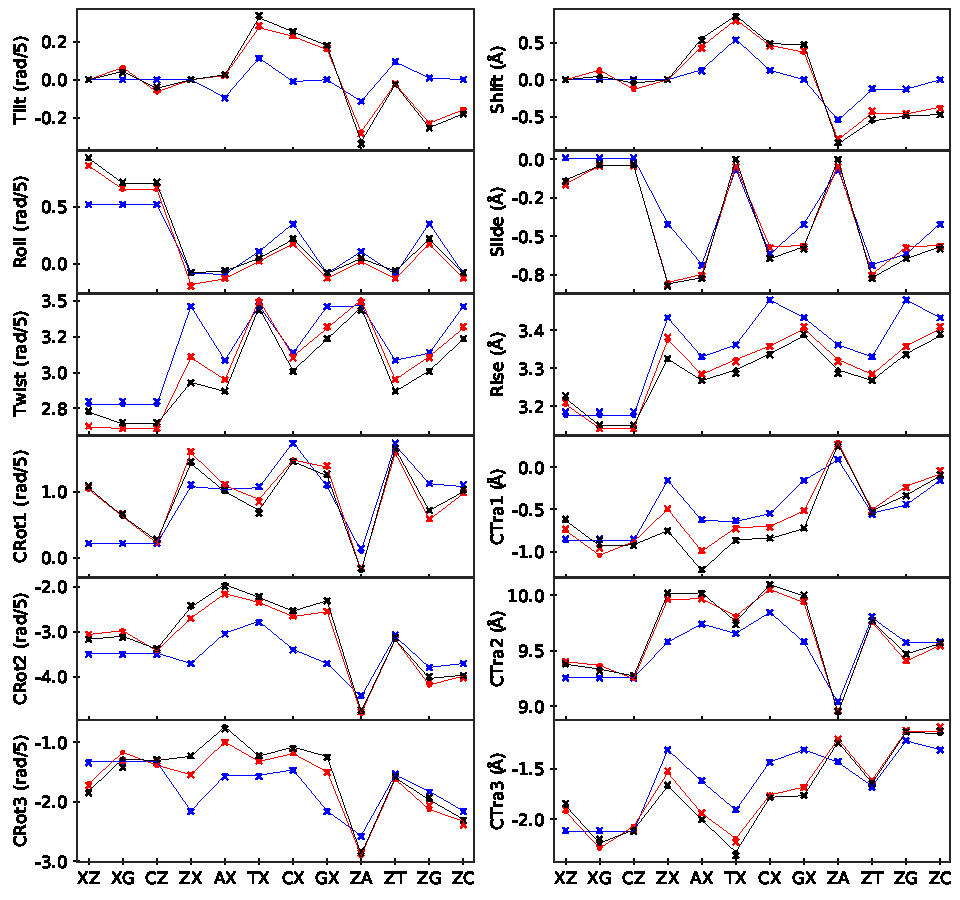
\includegraphics[width=15cm]{images/compare_dim_gs_DNA_MDNA_HDNA_gs.pdf}
\end{center}
\centering\caption{
Comparison of base-pair step coordinates for dsDNA where unmodified steps (X = C and Z = G) are in Blue, methylated steps (X = M and Z = N) are in Red, and hydroxymethylated steps (X = H and Z = K) are in Black. For each base-pair step, average coordinates observed in MD simulations and corresponding cgNA$+$ predictions are plotted in $\bullet$ and $\times$, respectively.
For better visualization, a line plot is plotted along $\bullet$.
}
\label{c6:fig3_dimercomp}
\end{figure}



In \cref{c6:fig5_seq_logo_sens}(a), we have plotted the findings when the central \cpg step was substituted by MN. 
It can be seen that sequences with the least change in groundstate have X$_1$,X$_2$ = A, G and Y$_1$,Y$_2$ = T, C alphabets to the upstream (left) and the downstream (right) of \cpg step, respectively, with information content $\approx$ 2.
If we read the sequence from both strands in $5^\prime-$ to $3^\prime-$ direction, there is a GA before C/M, implying a strong correlation between the least change in groundstate of the modified sequence and the presence of purines upstream to C.
Lastly, there is no information content for X$_3$, X$_4$, Y$_3$, and Y$_4$, indicating that beyond hexamer sequence does not influence the groundstate on epigenetic modifications.
Moreover, in the bottom plot, we have presented the information content in the sequences that are most influenced by the methylation of the central \cpg step.
The findings indicate that the maximum change in groundstate is correlated with the presence of C or G base-pairs adjacent to the central \cpg steps and A or T base-pairs at hexamer context.
\Cref{c6:fig5_seq_logo_sens}(b) is an analogous plot for the asymmetric methylation (MG) to the central \cpg step. 
The sequences with the least change in groundstate when \cpg step is substituted by either MG or MN are almost the same.
The similarities in the sequence logos include X$_1$ = A, X$_2$ = A or G, and Y$_1$ = T, whereas differences include no information at Y$_2$ (possibly because as Y$_2$ is away from M) and X$_3$ is more likely to be C or T (pyrimidine). 
In contrast, the sequences with maximum changes in groundstate due to asymmetric methylation are slightly different from those with symmetric methylation.
The sequence logos show a strong preference for T and G at X$_2$ and X$_1$, respectively, and A at Y$_1$, which can be explained by the fact that in asymmetric methylation, Y$_1$ position is, in fact, two base-pairs away from methylated C and can be considered as Y$_2$ which agrees with the sequence logos for symmetric methylation.
Lastly, the corresponding plots for \cpg step hydroxymethylation are almost identical as shown in \cref{c6:fig5_seq_logo_sens}(c) and (d).


\begin{figure}[H]
\begin{center}
 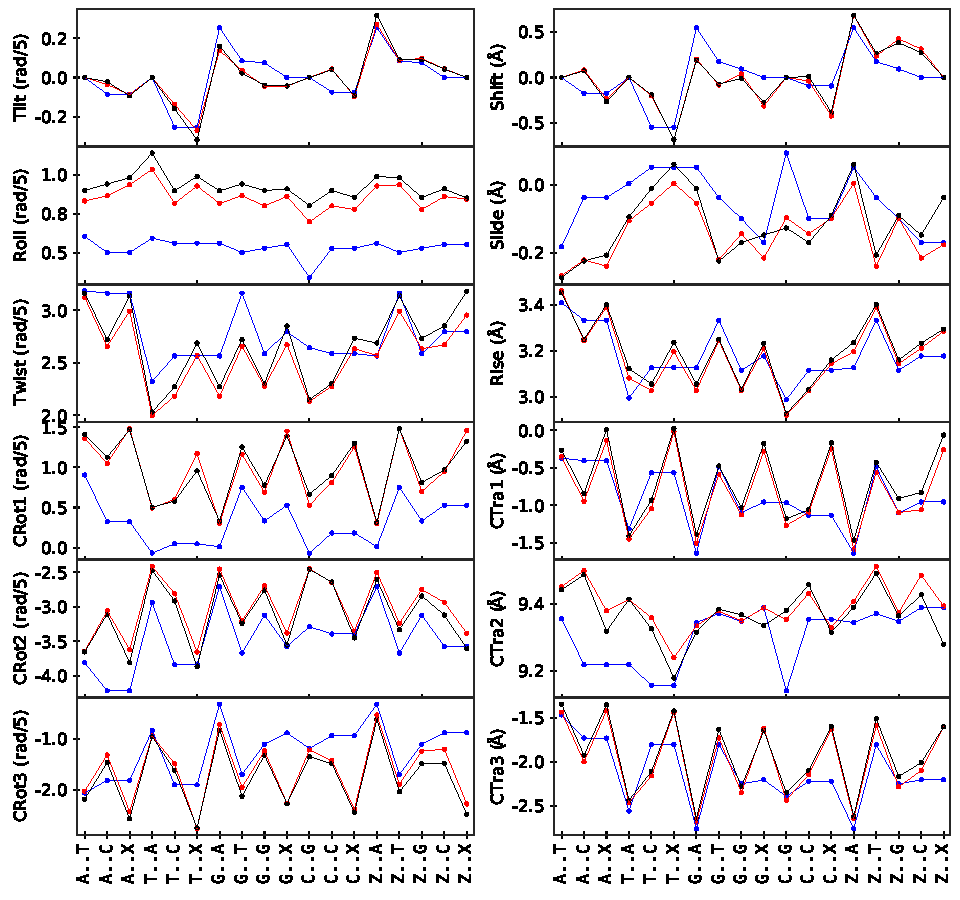
\includegraphics[width=15cm]{images/DNA_MDNA_HDNA_gs_MN_tet_context_gs.pdf}
\end{center}
\centering\caption{
Comparison of \cpg step coordinates in various flanking contexts where coordinates for unmodified, methylated, and hydroxymethylated \cpg steps are in blue, red, and black, respectively. X-axis are the flanking contexts where X = C and Z = G for unmodified \cpg steps, X = M and Z = N for methylated \cpg steps, X = H and Z = K for hydroxymethylated \cpg steps.
For better visualization, a line plot is plotted along $\bullet$.
}
\label{c6:fig4_tet_context}
\end{figure}
\clearpage

In summary, sequences with flanking A or T before modified cytosine (in \cpg step) are relatively inert to epigenetic modifications, whereas sequences with C or G before modified cytosine are highly sensitive. 
In the plots, we have shown statistics obtained from extreme 0.5\% sequences and using symmetric Mahalanobis distance as a metric; however, we would like to emphasize that the results are not sensitive to these choices.
Any other choices for metric (such as L$^1$-norm of the difference in groundstate) and outlier cut-off lead to similar conclusions.
Moreover, in \cref{c6:fig6_sensitivity}, we have plotted the groundstate for two sequences which only differ by immediate flanking context (underlined) to \cpg step, GCGTCGG\underline{AA}\textbf{CG}\underline{T}TTTGTCGGC and GCGTCGG\underline{TG}\textbf{CG}\underline{C}TTTGTCGGC to visualize the change in groundstate on the symmetric methylation of the central \cpg step (in bold). 
The change in groundstate for the latter sequence on  \cpg methylation is much larger and non-local compared to the former, particularly for the phosphate coordinates.

\begin{figure}[H]
\begin{center}
  \begin{subfigure}{7cm}
    \centering\includegraphics[width=7cm]{images/epi_sensitivity_groundstate_seq_logo_MN_MAHAL.pdf}
    \centering\caption{\cpg to MN}
  \end{subfigure}
  \begin{subfigure}{7cm}
    \centering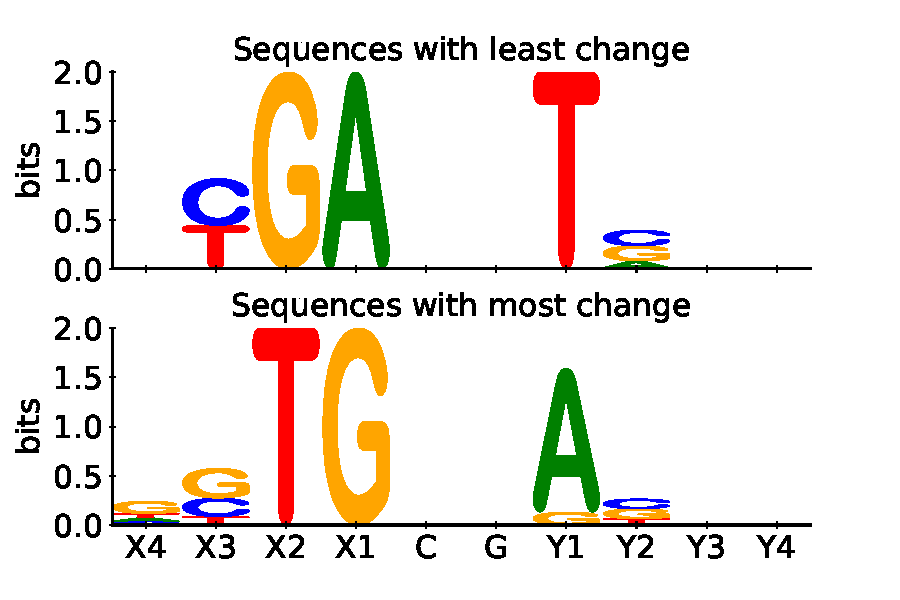
\includegraphics[width=7cm]{images/epi_sensitivity_groundstate_seq_logo_MG_Mahal.pdf}
    \centering\caption{\cpg to MG}
  \end{subfigure}

  \begin{subfigure}{7cm}
    \centering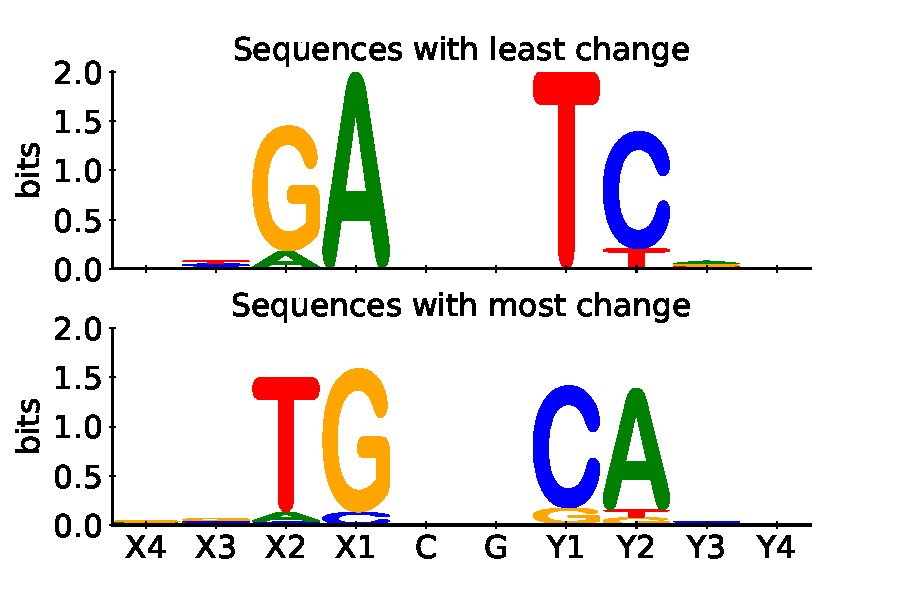
\includegraphics[width=7cm]{images/epi_sensitivity_groundstate_seq_logo_HK_Mahal.pdf}
    \centering\caption{\cpg to HK}
  \end{subfigure}
  \begin{subfigure}{7cm}
    \centering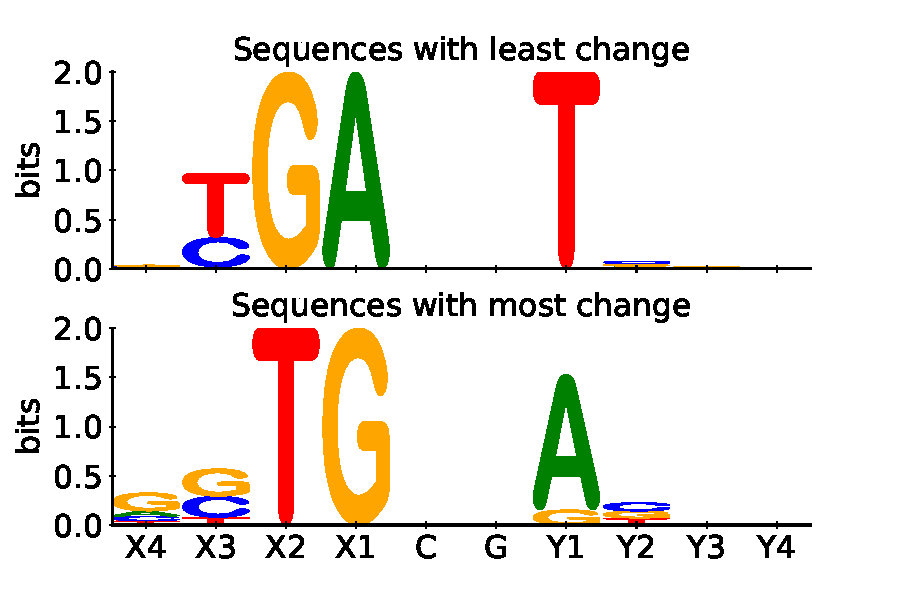
\includegraphics[width=7cm]{images/epi_sensitivity_groundstate_seq_logo_HG_Mahal.pdf}
    \centering\caption{\cpg to HG}
  \end{subfigure}
\centering\caption{Sequence logos to highlight flanking contexts that least and most influence the change in groundstate upon epigenetic modification of central \cpg step. Statistics are obtained from all decamers with central \cpg steps embedded in a 22mer, i.e.,  GCGTCGX$_4$X$_3$X$_2$X$_1$\textbf{CG}Y$_1$Y$_2$Y$_3$Y$_4$GTCGGC and information content in X$_j$ and Y$_j$ for most (top 0.5$\%$) and least change (bottom 0.5$\%$) in the groundstate are plotted on the ordinate.
}
\label{c6:fig5_seq_logo_sens}
\end{center}
\end{figure}

We want to highlight that the probability of occurrence of C or G base-pairs adjacent to \cpg step is much more likely in \cpg islands than in non-\cpg islands.
Traditionally, increased dsDNA stiffness due to epigenetic modifications is considered the controlling factor to act as a gene silencer~\cite{cortini2016physics,perez2012impact,portella2013understanding}.
It is believed that methylation of \cpg steps reduces dsDNA flexibility and therefore, reduces its ability to interact with transcription factors, modulates dsDNA accessibility, and makes them less prone to wrap around nucleosomes.
Here, we have shown that the change in the equilibrium shape, i.e., groundstate is also a contributing factor to the differential behavior of modified dsDNA, in particular, for \cpg islands.


\begin{figure}
  \begin{subfigure}{15cm}
    \centering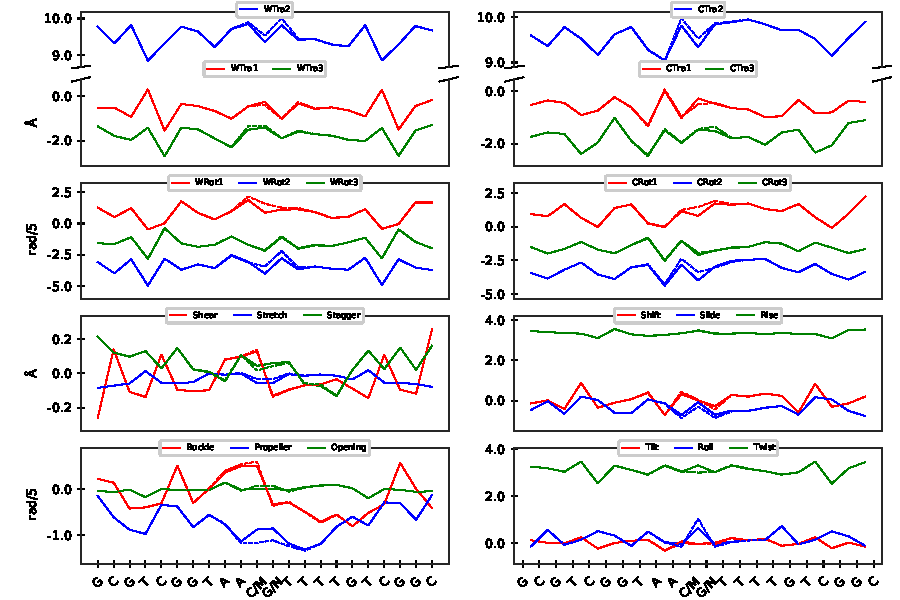
\includegraphics[width=15cm]{images/compare_epi_sensitivity_on_groundstate_MN_1.pdf}
    \centering\caption{Change in groundstate on symmetric methylation of central \cpg step}
  \end{subfigure} 
  
  \begin{subfigure}{15cm}
    \centering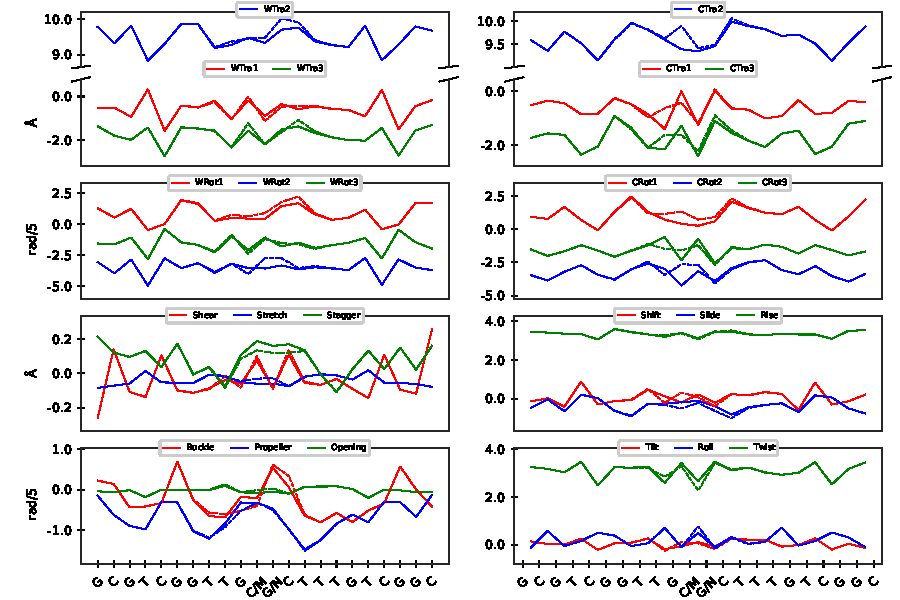
\includegraphics[width=15cm]{images/compare_epi_sensitivity_on_groundstate_MN_2.pdf}
    \centering\caption{Change in groundstate on symmetric methylation of central \cpg step}
  \end{subfigure}
\caption{Groundstate coordinates (elements of $w$) for (a) GCGTCGG\underline{AA}\textbf{CG}\underline{T}TTTGTCGGC (red, blue, and green as shown in legend) and same sequence with symmetric methylation on central \cpg step in dashed lines, and (b) groundstate coordinates for GCGTCGG\underline{TG}\textbf{CG}\underline{C}TTTGTCGGC (red, blue, and green as shown in legend) and same sequence with symmetric methylation on central \cpg step in dashed lines. 
The two sequences differ only in the immediate flanking sequence context (underlined) of the central \cpg step (in bold), and the figure highlights the role of flanking sequence context in the change of dsDNA groundstate upon \cpg methylation.}
\label{c6:fig6_sensitivity}
\end{figure}



% \section{\cpg islands}
% The human genome has approximately 42\% GC content, which implies that the probability of occurrence of a \cpg step is equal to $0.21\times 0.21 =0.0421$ or 4.21\%. 
% However, the observed frequency of \cpg steps is approximately five times less in human genomes. 
% \cpg islands are genomic regions with a high frequency of \cpg dinucleotides, often characterized by \cpg dinucleotide frequency greater than 60\% of statistically expected \cpg frequency.
% There are several closely related definitions of \cpg islands in the literature. 
% In this work, we have classified a sequence as \cpg islands if it follows the following three criteria defined in reference ~\cite{gardiner1987cpg}:
% \begin{itemize}
%     \item[a)] length of sequence must be greater than or equal to 200 bp,
%     \item[b)] GC content must be greater than 0.5,
%     \item[c)] observed to expected \cpg steps ratio must be greater than 0.6,
% \end{itemize}
% where GC content is defined as (number of G + number of C)/(length of sequence)  and expected \cpg steps is defined as (number of G * number of C)/(length of sequence).


% In this work, we have taken studied the effect of methylation and hydroxymethylation on the mechanics of \cpg islands.
% To do a systematic analysis, we have designed 
\section{Impact of epigenetic base modifications on groove widths}
As discussed earlier in \cref{c2:s4:sb4}, dsDNA displays a wide range of groove widths as a function of sequence; for example, minor groove widths range from 3 to 9 \AA.
The groove widths were computed for all decamers (~ one million) embedded in a flanking sequence of length six bps on both sides and taking central Watson phosphate (index 6 in decamer) as the reference phosphate.
Notably, we concluded from the sequence logos that the sequence alphabets at positions 2-6 in decamers influence the minor groove, and 4-10 influence the major groove. 

In limited prior studies exploring the influence of \cpg modification on groove widths, the observations are inconsistent. 
For instance, the general belief is that \cpg methylation narrows and widens the minor and major grooves, respectively~\cite{li2022dna,dantas2015evolving}.
However, a thorough analysis of available X-ray crystallographic and NMR data~\cite{rao2018systematic} has shown that the methylation of \cpg step may reduce or widen the minor groove depending on the sequence and location of the modified \cpg step.
%~\cite{kribelbauer2020toward}

In this section, we have investigated how epigenetic modifications of the \cpg step influence groove widths. 
Firstly, in \cref{c6:fig7_minor_groove}(a), we have plotted a schematic diagram of the CG base-pair showing that the methyl or hydroxymethyl (shown as X) is present in the major groove, thus, explicitly change the major groove chemical environment, while the minor groove remains the same.
For a systematic analysis of how this change affects the groove widths, we have performed two studies to explore the effect on groove widths due to (a) location of \cpg modification, and (b) extent of \cpg modification in the sequence. 
Note that we have used the same protocol described in \cref{c2:s4:sb4} for both studies.

For the first study, we have considered sequences of length 22 bps, i.e., GCTGTGX$_1$\textbf{X$_2$X$_3$}- \textbf{X$_4$X$_5$X$_6$}X$_7$X$_8$X$_9$X$_{10}$CATGGC and varied the position of \cpg step in \textbf{X$_2$X$_3$X$_4$X$_5$X$_6$} and computed the difference in groove widths before and after the modification of that \cpg step.
The results are plotted in \cref{c6:fig7_minor_groove}(b), showing that the minor grooves generally widen on \cpg step modification and depend on the position of the \cpg step. 
Moreover, the widening of the minor groove on \cpg modification is more for symmetric modifications than for asymmetric ones, and hydroxymethylation of \cpg step widens the minor groove more than methylation.
Lastly, the error bars in the plot are for various possible sequences by changing X$_i$s.

Furthermore, to investigate the influence on groove widths due to the extent of \cpg modifications, we have considered a sequence GCTGTG\textbf{CGCGCGCGCG}CATGGC of length 22 bp such that the central decamer is (CG)$_5$.
Then, we have iteratively modified (symmetric/asymmetric methylation/hydroxymethylation) this sequence by replacing one, two, three, four, and all five \cpg steps and computed the groove widths, and presented the findings in \cref{c6:fig7_minor_groove}. We have plotted minor groove widths with the percentage of \cpg modification, which shows a positive correlation between the minor groove widths and \% \cpg modification.
The minor groove width for a fully symmetrically methylated sequence is approximately one \AA \ larger than the corresponding unmodified sequence. \hfill \clearpage

\begin{figure}[H]
\begin{center}
  \begin{subfigure}{5.25cm}
    \centering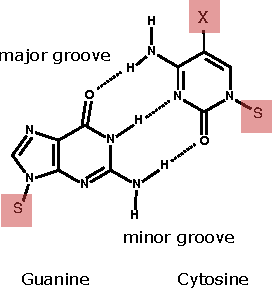
\includegraphics[width=4cm]{images/base-pair_mod.pdf}
    \caption{Grooves in modified CG base-pair}
  \end{subfigure}
  \begin{subfigure}{8.5cm}
    \centering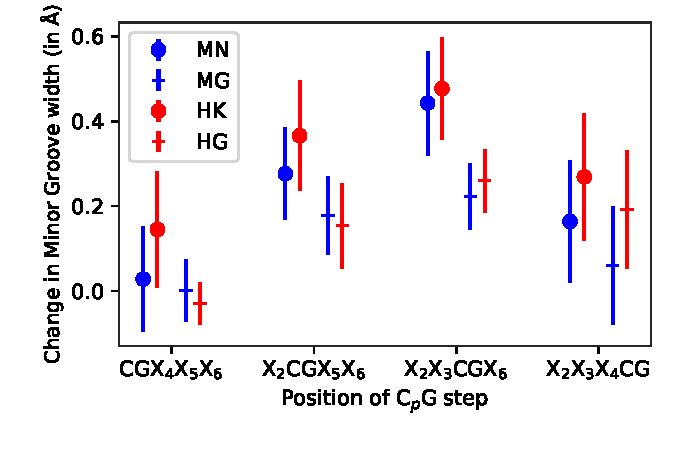
\includegraphics[width=7.5cm,trim=0.1cm 0.8cm 0cm 0.5cm]{images/modification_position_effect_minor_groove.pdf}
    \caption{Minor groove width on \cpg step modification}
  \end{subfigure}
  \begin{subfigure}{12cm}
    \centering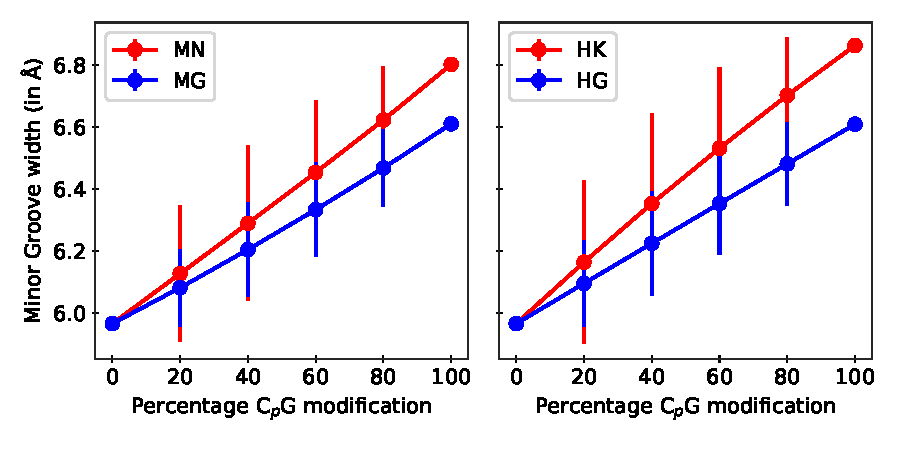
\includegraphics[width=10cm,trim=0.1cm 0.7cm 0cm 0.1cm]{images/modification_percent_effect_minor_groove.pdf}
    \centering\caption{Minor groove width on \% \cpg step modification}
  \end{subfigure}
\end{center}
\caption{
(a) Schematic diagram for grooves in modified CG base-pair where methyl/hydroxymethyl group (X) is in major groove.
Change in minor groove widths due to (b) \cpg modification at different positions in the highlighted sub-sequence of \linebreak GCTGTGX$_1$\textbf{X$_2$X$_3$}\textbf{X$_4$}\textbf{X$_5$X$_6$}X$_7$X$_8$X$_9$X$_{10}$CATGGC, and
(c) various extent of \cpg modification in the highlighted sub-sequence of GCTGTG\textbf{CG}\textbf{CG}\textbf{CG}\textbf{CG}\textbf{CG}CATGGC.
}
\label{c6:fig7_minor_groove}
\end{figure}

%left bottom right top

%%%%%%%%%%%%%%%%%%%%%%%%
%trim=left bottom right top,
\begin{figure}[H]
\begin{center}
\centering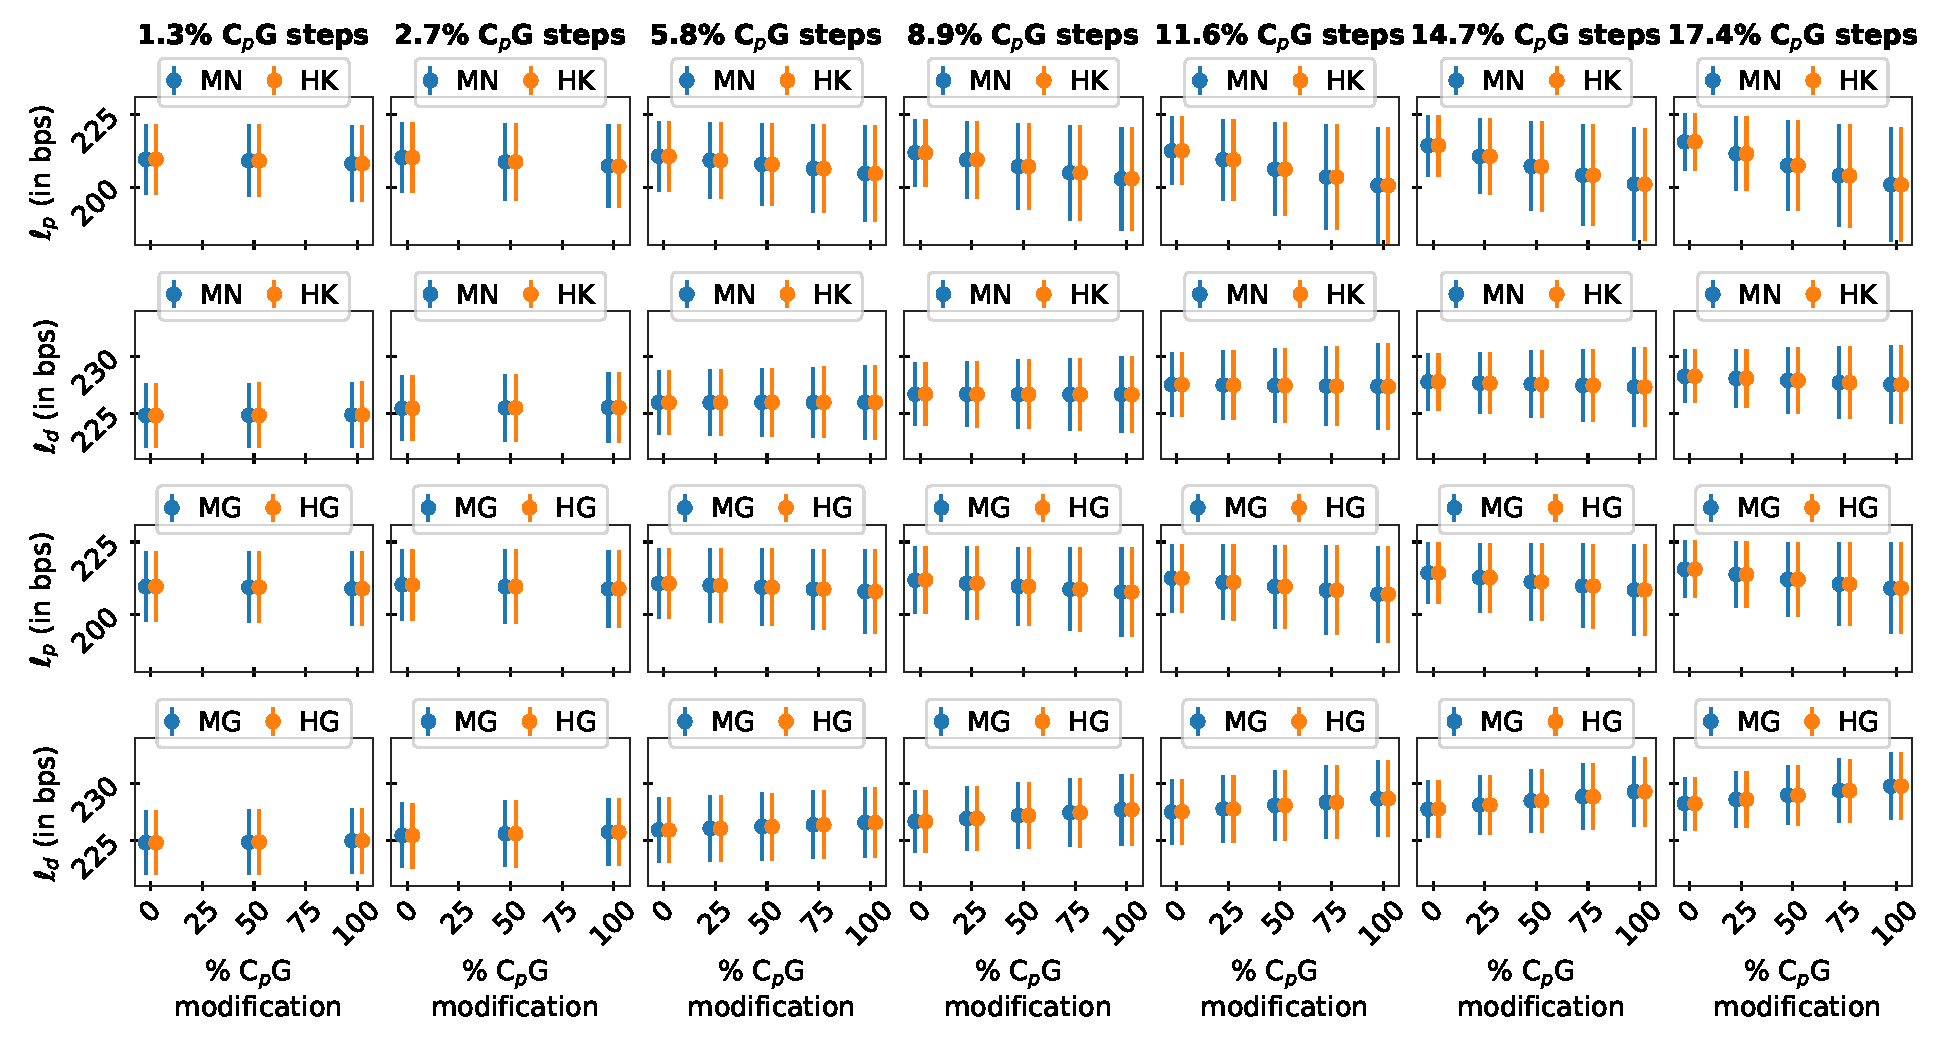
\includegraphics[width=15.5cm,trim=1.5cm 0.95cm 0cm 0.6cm]{images/persis_length_epi.pdf}
\end{center}
\caption{
Each subplot plots apparent ($\ell_{p}$) or dynamic ($\ell_{d}$) persistence lengths for sequences containing x\% \cpg steps (shown in title) for increasing \% randomly modified \cpg steps (shown in legend).
$\bullet$ and error bar are the mean and standard deviation for 20,000 random sequences.
}
\label{c6:fig7_persis}
\end{figure}
\noindent Similar trends are observed for asymmetric methylation of \cpg steps, but the range of variation is slightly smaller ($\approx$ 0.8 \AA).
Moreover, hydroxymethylation of \cpg steps has an almost identical effect on the minor groove widths. 
Also, we would like to highlight that the position of the modified \cpg step is crucial, as can be deduced from the error bar in the plot, in which sequences with the same percentage of \cpg step modification have different minor groove widths.

Lastly, \cpg modification slightly widens the major grooves. 
The plots are not shown here for brevity.
However, it must be noted that even though the major groove width does not change significantly on \cpg modification, it significantly changes the chemical environment inside the major grooves (with methyl group being hydrophobic while hydroxymethyl being hydrophilic) and therefore, has implications in protein-DNA interactions~\cite{rao2018systematic}. 

\section{Effect of \cpg modification on the persistence lengths of dsDNA} 
%One of the most popular and traditional measures for quantifying the rigidity of the NAs is persistence length, which can be defined as the length scale over which correlations in the direction of tangent along a polymer centerline are lost~\cite{hagerman1988flexibility}. 
In this work, we have computed sequence-dependent dynamic persistence length, $\ell_{d}$ by factoring out the contributions of the intrinsic shape from apparent persistence length $\ell_{p}$ as described in ref.~\cite{cgdnamc} and summarized in \cref{c2:sec6} in the context of the cgNA$+$ model.
Moreover, in \cref{c4:s5sb3}, we have shown that both the apparent and dynamic persistence lengths strongly depend on the sequence. 

A general consensus is that methylation leads to an increase in persistence length~\cite{hagerman1988flexibility,severin2011cytosine,perez2012impact,banyay2002structural}.
However, recent experimental studies~\cite{pongor2017optical,shon2019submicrometer} revealed that hypermethylation could increase dsDNA flexibility.
%shon2019submicrometer Increase in persistence length with \%GC content and on hypermethylation decrease in persistence length.. for less methylation, a slight increase. 
Therefore, to investigate the influence of \cpg modification on the persistence length of dsDNA, we conducted a systematic study for 0.5 million sequences of length 220 bps for each type of \cpg modification.
In particular, we have generated several lists of 20,000 sequences with different percentages of \cpg steps, namely, 1.3\%, 2.7\%, 5.8\%, 8.9\%, 11.6\%, 14.7\%, and 17.4\% and then randomly modified 0\%, 25\%, 50\%, 75\%, and 100\% of the \cpg steps.
In \cref{c6:fig7_persis}, we have plotted the dynamic and apparent persistence of all sequences.
Each subplot, from left to right, plots persistence length for sequences with increasing \%\cpg steps, and in each subplot, we have shown persistence length for sequences with different \%\cpg modification, i.e., 0\% and 100\% \cpg modification means unmodified and completely modified (\cpg steps) sequences.
Each data point is the mean and standard deviation of persistence length for 20,000 random sequences with a particular percentage of \cpg steps and a certain number of those \cpg steps are randomly modified.
The following observations can be made from \cref{c6:fig7_persis}:
\begin{itemize}
\item With an increase in \%\cpg steps in the sequence (which may also correspond to GC content) both $\ell_{p}$ and $\ell_{d}$ increase. 
\item The effects on persistence length for both modifications, methylation and hydroxymethylation, are almost similar.
\item According to the definition, $\ell_{d}-\ell_{p}>0$, but this difference increases with increasing \% modified \cpg steps. 
It implies that the modified \cpg steps make the intrinsic or groundstate shape of the sequence more bent, which might be attributed to the increased Roll of the \cpg steps (refer to \cref{c6:fig4_tet_context}).
\item The symmetric and asymmetric modifications show a similar pattern  for $\ell_{p}$, i.e, $\ell_{p}$ decreases when \% modification increases.  
Moreover, the decrease in $\ell_{p}$ also depends on the number of \cpg steps in the sequence, since more modified \cpg steps lead to a further decrease in $\ell_{p}$.
\item Whereas, $\ell_{d}$ remains constant on symmetric modification and $\ell_{d}$ increases when \% asymmetric modification increases. 
\end{itemize}
Thus, by rigorous computations, we found that the apparent persistence length of a given sequence decreases with the \cpg step modification, while the dynamic persistence length remains almost similar for symmetric modification and increases for asymmetric modification.